\documentclass{ds-report}

\usepackage[T1]{fontenc}
\usepackage{graphicx}
\usepackage{lmodern}
\usepackage{lscape}

\assignment{Java RMI} % Set to `Java RMI`, `Java EE` or `Google App Engine`.
\authorOne{Thomas Bamelis} % Name of first team partner.
\studentnumberOne{r0640219} % Student number of first team partner.
\authorTwo{Michiel Jonckheere} % Name of second team partner.
\studentnumberTwo{r0665594}  % Student number of second team partner.

\begin{document}
	\maketitle

	\paragraph{Question 1} 
	The client looks up information he needs for making a quote. When a client make a quote with certain constraints, it asks for a quote to the car rental agency who returns the first available quote at one of the registered car companies. 
	The client can do this for a number of quotes, which are all saved to his session. When the client wants to confirm his quotes, he notifies the car rental agency. The car rental agency tries to confirm all quotes at the relevant car rental companies. If one fails, the already confirmed reservations are cancelled and the client is notified of the failure.
	
	
	\paragraph{Question 2}
	If an object of the class must be sent over the wire, the class must be serializable. This interface streams the object into a sequence of bytes and the receiver can restore the bytestream to the object. So each parameter or return value of remote methods must be serializable  (so also when it is contained in an object which has to be serializable). E.g. we had to make the class CarType serializable. 
	
	
	\paragraph{Question 3} 
	When a remote process wants to call a method on a local object. 
	als ze methods bevatten die remotely callable zijn. de interface extends van Remote, de klasse implementeerd die, zoals ICarRentalAgency en CarRentalAgency.
	
	\paragraph{Question 4}
	The data to be transmitted between client and server and back are the arguments and the return value of the remote call. In this case it has to be a string that contains the name of the client and the return will be an integer which contains the number of reservations of the specific renter.
	
	\paragraph{Question 5} TODO diagram~\\
	
	
	%First the client to CRA communication:\\
	The client and CRA are on a different server. The client uses a CRA-stub which it looks up on a registry on the CRA-server to receive manager and reservation session-stubs. Interacting with the CRA is then done through this sessions. Every session on the client is a remote interface for a session object on the CRA-server. The session object then interacts locally with the CRA-object on the CRA-server. \\
	
	All interaction run through the CRA-object and the client never directly talks to a CRC. \\
	
	The CRA interacts with different CRC's which are all on their own remote servers. The CRA uses an interface to a remote CRC-object when interaction is necessary. The CRA keeps a list of interfaces of the registered CRC's. The only registry is located on the CRA and everybody interacts with it. When a CRC wants to register itself it pushes itself to this remote registry and notifies the CRA through a managersession. 
	
	\paragraph{Question 6} 
	The CRA uses a hashmap with as key the name of the company and as value an interface stub to the remote object. A CRC pushes itself on to the registry before notifing the CRA with the name by which it can lookup the interface.\\
	
	TODO why did we choose this approach???
	
	\paragraph{Question 7} 
	When a session is created it is created on the CRA-server and it pushes itself to registry. The CRA-server then sends the lookup name to the client for it to be used. When the client is done with the session, he calls close session on the remote interface to the remote object. The remote object then removes itself from the registry, thus removing the last local reference to it causing de garbage collector to collect the session. \\
	
	TODO why did we choose this approach???
	
	\paragraph{Question 8} 
	Java RMI doesn't create copies of instances, so if an object is accessed by multiple clients, they all use the same object. That's why the objects that can be accessed by multiple threads must be made thread-safe.\\
	
	
	When a write is done, which is a change to a CRC-object, the CRA blocks any other call. So it's impossible for bad read to happen this way. Blocking is only necessary when quotes are being confirmed. We chose this approach because if the client can read incorrect information, he will e.g. be able to create invalid quotes. These will result in errors and the client will have to recall his methods to check which cartypes actually are available. 
	
	\paragraph{Question 9} 
	The scalability is affected in that only one client can confirm at a time and while confirming no other clients can do something. When there would be a lot of clients, this could be a potential bottleneck. 
	
	\clearpage
	
	% You can include diagrams here.
	
	\begin{landscape}
		\begin{figure}
			\centering
			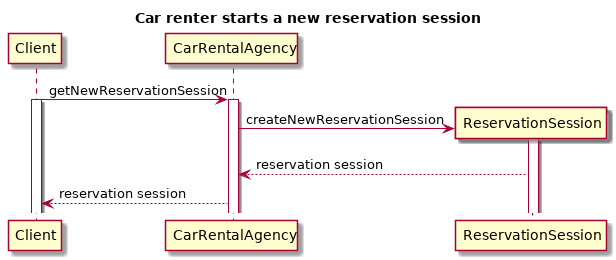
\includegraphics[width=\paperwidth]{../diagrams/sequenceDiagrams/startSession.png}
		\end{figure}
	\end{landscape}
	
\clearpage
	\begin{landscape}
		\begin{figure}
			\centering
			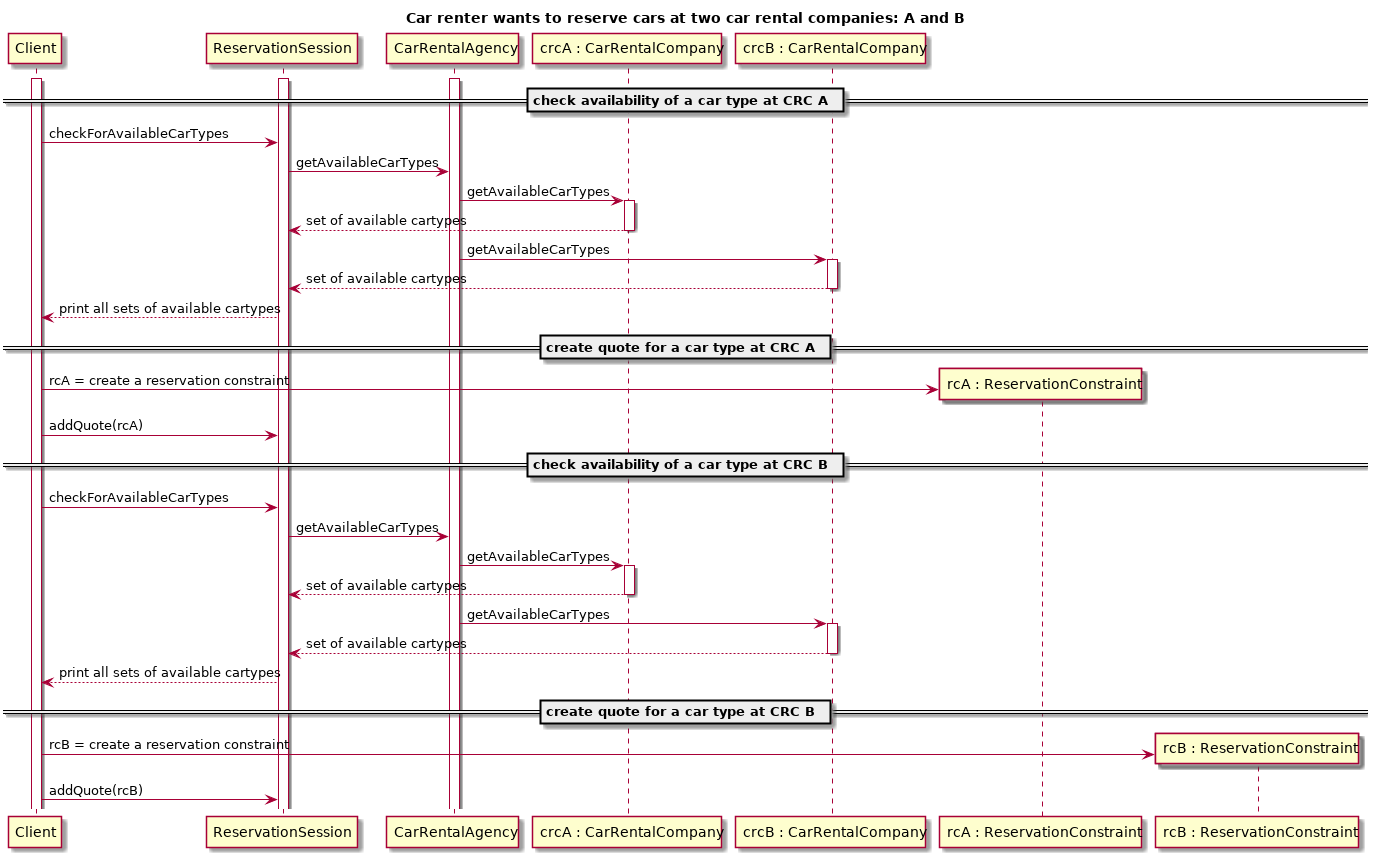
\includegraphics[width=\paperwidth]{../diagrams/sequenceDiagrams/reserveCars.png}
		\end{figure}
	\end{landscape}
	
\clearpage
	\begin{landscape}
		\begin{figure}
			\centering
			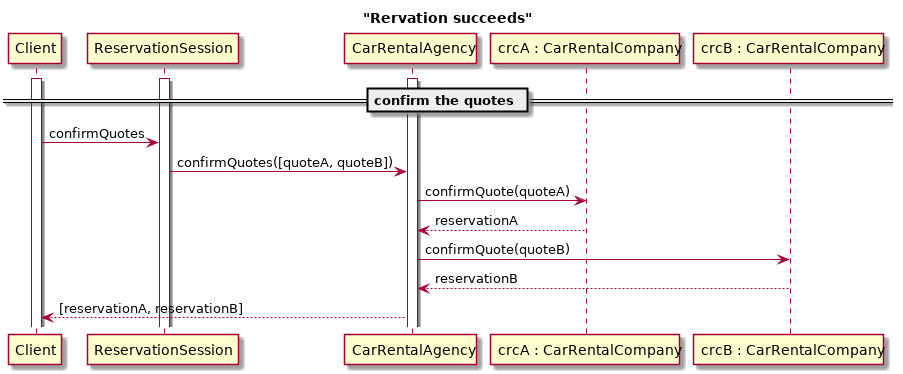
\includegraphics[width=\paperwidth]{../diagrams/sequenceDiagrams/reservationSucceeds.png}
		\end{figure}
	\end{landscape}
\clearpage
	\begin{landscape}
		\begin{figure}
			\centering
			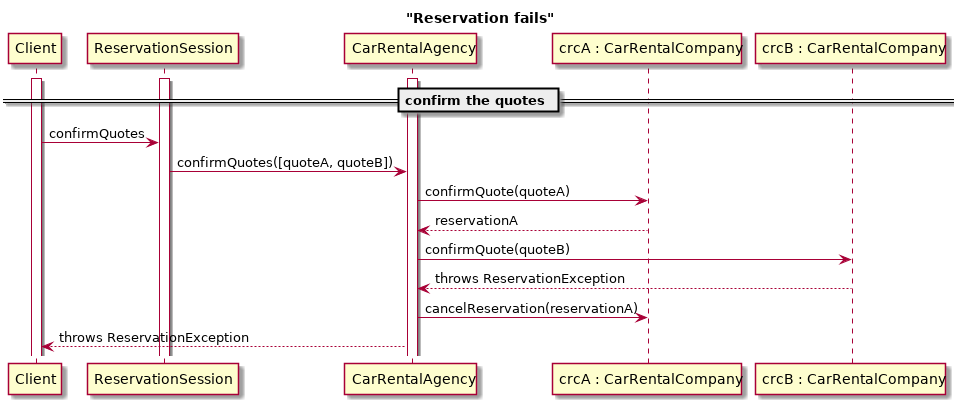
\includegraphics[width=\paperwidth]{../diagrams/sequenceDiagrams/reservationFails.png}
		\end{figure}
	\end{landscape}

\end{document}
